\subsection{Making Pycket an Independent Self-Hosting Racket}
\label{subsec:pycket}

Pycket is first designed in 2014 as a high-performance JIT compiler
for Racket, generated using the RPython meta-tracing framework
\cite{bolz14-racket}. The language interpreter is based on the CEK
abstract machine and has the state $\langle e, \rho, \kappa \rangle$ ($e$ : control
(program AST), $\rho$ : environment, $\kappa$ : continuation)
\cite{felleisen87}. \figref{fig:cek} shows the transition rules and
how the CEK-loop is implemented in Pycket. The interpreter loop
continuously reduces the CEK triple until an empty continuation is
reached, which triggers a \emph{Done} exception that returns the
results.

\begin{figure}[h!]
  \small
\begin{align*}
e &::= x \mid \lambda x.\, e \mid e \; e\\
\kappa &::= [] \mid \mathsf{arg}(e,\rho){::}\kappa \mid \mathsf{fun}(v,\rho){::}\kappa
\end{align*}
\begin{align*}
\langle x, \rho, \kappa \rangle & \longmapsto
    \langle \rho(x), \rho, \kappa \rangle \\
\langle (e_1 \; e_2), \rho, \kappa \rangle & \longmapsto
    \langle e_1, \rho, \mathsf{arg}(e_2, \rho){::}\kappa \rangle \\
\langle v, \rho, \mathsf{arg}(e,\rho'){::}\kappa \rangle & \longmapsto
    \langle e, \rho', \mathsf{fun}(v,\rho){::}\kappa \rangle \\
\langle v, \rho, \mathsf{fun}(\lambda x. \, e, \rho'){::}\kappa \rangle & \longmapsto
    \langle e, \rho'[x\mapsto v], \kappa \rangle
\end{align*}
\begin{lstlisting}[mathescape]
                                    try:
                                      while True:
                                        ast, env, cont = ast.interpret(env, cont)
                                    except Done, e:
                                      return e.values
\end{lstlisting}
\caption{The CEK Machine transitions and the loop in Pycket. Figure taken from \cite{pycket15}.}
\label{fig:cek}
\end{figure}

In its original design, as shown in \figref{fig:old-pycket}, Pycket
relies on the Racket executable to read and fully expand a given
module\cite{samth:11}, and then generates RPython AST for it and
evaluates it within the interpreter loop \cite{pycket15}. Exploiting
the increased portability in Racket, here we turn the Pycket from
being a rudimentary compiler to an actual implementation of Racket,
independent of the Racket executable.

\begin{figure}[h!]
  \centering 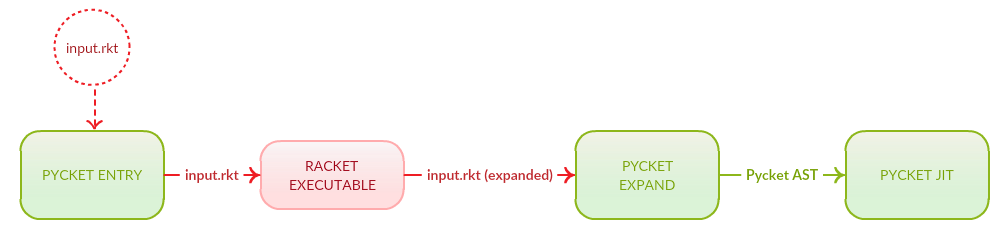
\includegraphics[scale=0.3]{img/old-pycket-2}
\caption{Pycket used to run Racket's executable to fully expand a given module before running it.}
\label{fig:old-pycket}
\end{figure}

First step is building the \emph{linklets} layer by implementing the
\emph{compile-linklet} and \emph{instantiate-linklet} functions in
RPython, thereby allowing Pycket to process and evaluate linklets. The
\emph{compile-linklet} takes an s-expression for a linklet to produce
a linklet object as described in
\secref{subsec:linklets-semantics}. It makes several passes on the
s-expression to determine the identifiers that are defined within the
linklet and the ones that are mutated. Then it processes the imported
and exported identifiers to produce the Import and Export run-time
objects, freshly generating identifiers (gensym) as needed. Then it
makes a final recursive pass to produce the RPython AST for the body,
and puts all the information within a linklet object. The
\emph{instantiate-linklet} on the other hand, carries out the steps
for running a linklet object. First it processes the Import and Export
objects and collects and creates variables as necessary, and prepares
the target instance (i.e. creates a new instance if it's a regular
instantiation) and interprets the body, effectively implementing the
$\longrightarrow_{\beta p}$ reduction in the \figref{fig:reduction} which will be
transitively applied by the interpreter loop.

After implementing the \emph{compile-linklet} and
\emph{instantiate-linklet}, the next step is to load the bootstrapping
linklets into the run-time as described in
\secref{subsec:racket-expand}. For simplicity, we are only concerned
with loading the \emph{expander} linklet, as it's the most essential
one for bootstrapping (also it's the biggest one). Loading the other
linklets are essentially the same process (modulo the run-time support
they need).

\begin{figure}[h!]
  \centering
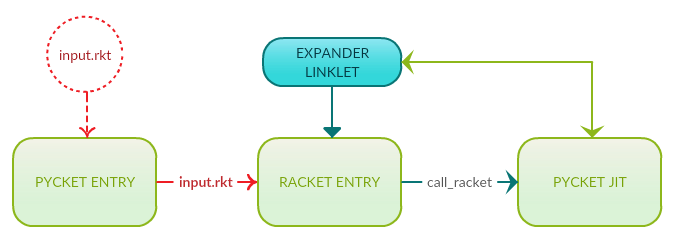
\includegraphics[scale=0.3]{img/new-pycket}
\caption{Pycket now uses the functionalities from the expander linklet to expand and run a given module.}
\label{fig:new-pycket}
\end{figure}

As we described in \secref{subsec:racket-expand}, the expander linklet
is generated offline by running the expander on itself using the
Racket's executable, and serialized as an s-expression. Pycket, then
reads this s-expression and runs \verb|compile-linklet| to produce a
linklet object, which is then instantiated using the
\verb|instantiate-linklet|, and the functions from the expander
linklet is load into the run-time. At this point, Pycket has all the
functionalities implemented and exported by the expander, such as
read, expand, eval etc., in its run-time to call.

%\begin{lstlisting}[mathescape]
\begin{minted}[numbersep=0pt,gobble=0,linenos,numbers=left,fontsize=\footnotesize,frame=lines]{python}
    expander_linklet_obj = compile_linklet([expander_linklet_sexp, ...])
    expander_linklet_instance = instantiate_linklet([expander_linklet_obj, ...])
    expander_linklet_instance.expose_vars_to_prim_env()
\end{minted}

Having the expander and all the functions that it provides in its
run-time allows Pycket to run a wide variety of Racket programs and
easily implement run-time functionalities. For example, a very simple
implementation of our running example top-level repl can directly use
Racket's read, expand and eval functions, as shown in
\figref{fig:repl-rpython}. The \verb|call_racket| is a wrapper that
handles the setup to call Racket functions within the CEK loop.

\begin{wrapfigure}[8]{r}{0.42\textwidth}
  \vspace{-0.6cm}
\begin{minted}[numbersep=0pt,gobble=0,linenos,numbers=left,fontsize=\footnotesize,frame=lines]{python}
  while True:
    r_exp = read.call_racket([repl.readline(), ...])
    r_expanded = expand.call_racket([r_exp, ...])
    result = eval.call_racket([r_expanded, ...])
    print(result)
\end{minted}
\caption{hede}
\label{fig:repl-rpython}
\end{wrapfigure}

Moreover, since the expander provides the implementations of Racket's
macro-system and the module-system, Pycket is able to run programs
that are in languages built on top of Racket core, such as
\emph{racket/base}. Therefore, instead of implementing the top-level
repl itself, Pycket can directly run Racket's own repl, which is
implemented as a \emph{racket/base} program, through the
\verb|dynamic-require| function exported by the expander.

%\begin{minted}[numbersep=0pt,gobble=0,linenos,numbers=left,fontsize=\footnotesize,frame=lines]{python}
{\footnotesize
\begin{lstlisting}[mathescape]
  dynamic_require.call_racket(['racket/repl,'read-eval-print-loop])
\end{lstlisting}
}
%\end{minted}

These programs, including the bootstrapping linklets themselves often
require additional run-time support such as \emph{correlated} objects
(which are syntax objects without the lexical-content information),
Racket-level exception handling and primitive functions. For example,
running Racket's repl requires delimited continuations. Also handling
exceptions in Racket code in the run-time requires Racket-level
exception handling on Pycket. The existing Pycket implementation has a
rudimentary exception handling mechanism via transforming the
Racket-level exceptions (which are implemented by Racket structs) into
the RPython exceptions. However, having Racket-level exceptions
requires the run-time to support installing Racket-level handlers via
continuation-marks and dynamically pass the Racket-level exceptions to
the appropriate handlers.

Moreover, the Racket itself (including the bootstrapping linklets)
generally relies on a large number ($\sim$1500) of primitives, aroud 900
of which we already have in the existing Pycket implementation. An
additional $\sim$200 primitives need to be implemented, along with the
addition of the run-time liblaray \texttt{\#\%linklet} that will
contain 32 linklet related functions including the
\emph{compile-linklet}, \emph{instantiate-linklet} and
\emph{instance-variable-value}.

\subsubsection{More On Portability}
\label{subsec:more-portability}

One of the essential nuances of self-hosting Racket with the expander
linklet, is that the interaction between the run-time and the expander
is a two-way street. The VM implements and uses \verb|compile-linklet|
and \verb|instantiate-linklet| to import the functions provided by the
expander, and the expander provides functions that uses the
\verb|compile-linklet| and \verb|instantiate-linklet| functions, along
with the other run-time primitives as well.

For example, the \verb|dynamic-require| used above (provided by the
expander linklet) is a Racket function that dynamically loads a Racket
module (if it's not already loaded) by resolving the module path,
finding the source code in the file system, reading and expanding the
codes and modifying the namespace registry. The Racket code inside the
expander that implements all that calls run-time primitives such as
for file-system support and also calls the \verb|compile-linklet| and
\verb|instantiate-linklet| for expanding and instantiating all the
required modules. Another example is the \verb|eval| function as we
discussed in \secref{subsec:portability}.

This intertwined nature of the high-level language facilities and the
low-level run-time support is central to the Racket's improved
portability.
